% Template of basic phisics experiment 基于 article template, 在此基础上做修改
% 设定文章编码类型, 正文字号为五号则 zihao=5, 正文字号为小四则 zihao=-4
\documentclass[zihao=5, UTF8]{article}		


% 自定义宏定义
\def\N{\mathbb{N}}
\def\F{\mathbb{F}}
\def\Z{\mathbb{Z}}
\def\Q{\mathbb{Q}}
\def\R{\mathbb{R}}
\def\C{\mathbb{C}}
\def\T{\mathbb{T}}
\def\S{\mathbb{S}}
\def\A{\mathbb{A}}
\def\I{\mathscr{I}}
\def\d{\mathrm{d}}
\def\p{\partial}


% 物理实验报告所需的其它宏包
\usepackage{ulem}   % \uline 下划线支持

% 导入基本宏包
\usepackage[UTF8]{ctex}     % 设置文档为中文语言
\usepackage[colorlinks, linkcolor=blue, anchorcolor=blue, citecolor=blue, urlcolor=blue]{hyperref}  % 宏包: 自动生成超链接 (此宏包与标题中的数学环境冲突)
% \usepackage{docmute}    % 宏包: 子文件导入时自动去除导言区, 用于主/子文件的写作方式, \include{./51单片机笔记}即可. 注: 启用此宏包会导致.tex文件capacity受限. 
\usepackage{amsmath}    % 宏包: 数学公式
\usepackage{physics}
\usepackage{bm}
\usepackage{mathrsfs}   % 宏包: 提供更多数学符号
\usepackage{amssymb}    % 宏包: 提供更多数学符号
\usepackage{pifont}     % 宏包: 提供了特殊符号和字体
\usepackage{extarrows}  % 宏包: 更多箭头符号
\usepackage{multirow}
\usepackage{siunitx}

\renewcommand{\dd}{\mathrm{d}}

% 列表环境设置
\usepackage{enumitem}   % 宏包: 列表环境设置
    \setlist[enumerate]{itemsep=0pt, parsep=0pt, topsep=0pt, partopsep=0pt, leftmargin=3.5em} 
    \setlist[itemize]{itemsep=0pt, parsep=0pt, topsep=0pt, partopsep=0pt, leftmargin=3.5em}
    \newlist{circledenum}{enumerate}{1} % 创建一个新的枚举环境  
    \setlist[circledenum,1]{  
        label=\protect\circled{\arabic*}, % 使用 \arabic* 来获取当前枚举计数器的值, 并用 \circled 包装它  
        ref=\arabic*, % 如果需要引用列表项, 这将决定引用格式（这里仍然使用数字）
        itemsep=0pt, parsep=0pt, topsep=0pt, partopsep=0pt, leftmargin=3.5em
    }  
% 文章页面 margin 设置
\usepackage[a4paper]{geometry}  % 宏包: 文章页面 margin 设置
    \geometry{top=0.75in}
    \geometry{bottom=0.75in}
    \geometry{left=0.75in}
    \geometry{right=0.75in}   % 设置上下左右页边距
    \geometry{marginparwidth=1.75cm}    % 设置边注距离（注释、标记等）

% 自定义数学环境
\usepackage{amsthm} % 宏包: 数学环境配置
% theorem-line 环境自定义
    \newtheoremstyle{MyLineTheoremStyle}% <name>
        {11pt}% <space above>
        {11pt}% <space below>
        {}% <body font> 使用默认正文字体
        {}% <indent amount>
        {\bfseries}% <theorem head font> 设置标题项为加粗
        {: }% <punctuation after theorem head>
        {.5em}% <space after theorem head>
        {\textbf{#1}\thmnumber{#2}\ \ (\,\textbf{#3}\,)}% 设置标题内容顺序
    \theoremstyle{MyLineTheoremStyle} % 应用自定义的定理样式
    \newtheorem{LineTheorem}{Theorem.\,}
% theorem-block 环境自定义
    \newtheoremstyle{MyBlockTheoremStyle}% <name>
        {11pt}% <space above>
        {11pt}% <space below>
        {}% <body font> 使用默认正文字体
        {}% <indent amount>
        {\bfseries}% <theorem head font> 设置标题项为加粗
        {: \\ \indent}% <punctuation after theorem head>
        {.5em}% <space after theorem head>
        {\textbf{#1}\thmnumber{#2}\ \ (\,\textbf{#3}\,)}% 设置标题内容顺序
    \theoremstyle{MyBlockTheoremStyle} % 应用自定义的定理样式
    \newtheorem{BlockTheorem}[LineTheorem]{Theorem.\,} % 使用 LineTheorem 的计数器
% definition 环境自定义
    \newtheoremstyle{MySubsubsectionStyle}% <name>
        {11pt}% <space above>
        {11pt}% <space below>
        {}% <body font> 使用默认正文字体
        {}% <indent amount>
        {\bfseries}% <theorem head font> 设置标题项为加粗
        {: \\ \indent}% <punctuation after theorem head>
        {0pt}% <space after theorem head>
        {\textbf{#3}}% 设置标题内容顺序
    \theoremstyle{MySubsubsectionStyle} % 应用自定义的定理样式
    \newtheorem{definition}{}


% 有色文本框及其设置
\usepackage[dvipsnames,svgnames]{xcolor}    %设置插入的文本框颜色
\usepackage[strict]{changepage}     % 提供一个 adjustwidth 环境
\usepackage{framed}     % 实现方框效果
    \definecolor{graybox_color}{rgb}{0.95,0.95,0.96} % 文本框颜色. 修改此行中的 rgb 数值即可改变方框纹颜色, 具体颜色的rgb数值可以在网站https://colordrop.io/ 中获得. （截止目前的尝试还没有成功过, 感觉单位不一样）（找到喜欢的颜色, 点击下方的小眼睛, 找到rgb值, 复制修改即可）
    \newenvironment{graybox}{%
    \def\FrameCommand{%
    \hspace{1pt}%
    {\color{gray}\small \vrule width 2pt}%
    {\color{graybox_color}\vrule width 4pt}%
    \colorbox{graybox_color}%
    }%
    \MakeFramed{\advance\hsize-\width\FrameRestore}%
    \noindent\hspace{-4.55pt}% disable indenting first paragraph
    \begin{adjustwidth}{}{7pt}%
    \vspace{2pt}\vspace{2pt}%
    }
    {%
    \vspace{2pt}\end{adjustwidth}\endMakeFramed%
    }

% 各级标题自定义设置
\usepackage{titlesec}   
    % section标题自定义设置 
    \titleformat{\section}[hang]{\normalfont\huge\bfseries\centering}{第\,\thesection\,部分}{20pt}{}
    % subsection标题自定义设置 
    \titleformat{\subsection}[hang]{\normalfont\Large\bfseries}{\,\thesubsection\,}{8pt}{}
    % subsubsection标题自定义设置
    \titleformat{\subsubsection}[hang]{\normalfont\large\bfseries}{\,\thesubsubsection\,}{6pt}{}

% 外源代码插入设置
\usepackage{matlab-prettifier}
    \lstset{
        style=Matlab-editor,  % 继承matlab代码颜色等
    }
\usepackage[most]{tcolorbox} % 引入tcolorbox包 
\usepackage{listings} % 引入listings包
    \tcbuselibrary{listings, skins, breakable}
    \lstdefinestyle{matlabstyle}{
        language=Matlab,
        basicstyle=\small,
        breakatwhitespace=false,
        breaklines=true,
        captionpos=b,
        keepspaces=true,
        numbers=left,
        numbersep=15pt,
        showspaces=false,
        showstringspaces=false,
        showtabs=false,
        tabsize=2
    }
    \newtcblisting{matlablisting}{
        arc=0pt,
        top=0pt,
        bottom=0pt,
        left=1mm,
        listing only,
        listing style=matlabstyle,
        breakable,
        colback=white   % 选一个合适的颜色
    }

% table 支持
\usepackage{booktabs}   % 宏包: 三线表
\usepackage{tabularray} % 宏包: 表格排版
\usepackage{longtable}  % 宏包: 长表格

% figure 设置
\usepackage{graphicx}  % 支持 jpg, png, eps, pdf 图片 
\usepackage{svg}       % 支持 svg 图片
    \svgsetup{
        % 指向 inkscape.exe 的路径
        inkscapeexe = C:/aa_MySame/inkscape/bin/inkscape.exe, 
        % 一定程度上修复导入后图片文字溢出几何图形的问题
        inkscapelatex = false                 
    }


% 图表进阶设置
\usepackage{float}     % 图表位置浮动设置 
\usepackage{caption}    % 图注、表注
    \captionsetup[figure]{name=图}  
    \captionsetup[table]{name=表}
    \captionsetup{labelfont=bf, font=small}

%% 文章默认字体设置
%    \usepackage{fontspec}   % 宏包: 字体设置
%        \setmainfont{SimSun}[
%            BoldFont = SimHei, % 设置粗体字为黑体
%            ItalicFont = KaiTi, % 设置斜体字为楷体
%            BoldItalicFont = KaiTi % 设置粗斜体字为楷体
%        ] 
%        %\setCJKmainfont[AutoFakeBold=3]{SimSun} % 设置加粗字体为 SimSun 族, AutoFakeBold 可以调整字体粗细
%        \setmainfont{Times New Roman} % 设置英文字体为Times New Roman


% 其它设置
    % equation 公式编号设置
        \makeatletter  
        \renewcommand{\theequation}{\thesection.\arabic{equation}}  
        \makeatother
    % 脚注设置
        \renewcommand\thefootnote{\ding{\numexpr171+\value{footnote}}}
    % 参考文献引用设置
        \bibliographystyle{unsrt}   % 设置参考文献引用格式为unsrt
        \newcommand{\upcite}[1]{\textsuperscript{\cite{#1}}}     % 自定义上角标式引用
    % 文章序言设置
        \newcommand{\cnabstractname}{序言}
        \newenvironment{cnabstract}{%
            \par\Large
            \noindent\mbox{}\hfill{\bfseries \cnabstractname}\hfill\mbox{}\par
            \vskip 2.5ex
            }{\par\vskip 2.5ex}


% 页眉页脚设置
\usepackage{fancyhdr}   %宏包: 页眉页脚设置
    \pagestyle{fancy}
    \fancyhf{}
    \cfoot{\thepage}
    \renewcommand\headrulewidth{1pt}
    \renewcommand\footrulewidth{0pt}
    \rhead{\bfseries 分组序号: 3-04-1}    
    \chead{《基础物理实验》实验报告,\ 潘天麟\ 2023K8009908023}
    \lhead{2024.11.27}

\usepackage{pdfpages}

% 开始编辑文章

\begin{document}
\noindent\begin{flushright}
    \zihao{2}{分组序号: 3-04-1}
\end{flushright}

\newcommand*{\boldsong}{\CJKfamily{boldsong}}


\begin{center}\large
    \noindent{\Huge\bfseries\boldsong《基础物理实验》实验报告 }
    \\\vspace{0.4cm}
    \noindent\textit{
        \textbf{\boldsong 实验名称: }\uline{\hspace{2.3cm} 气轨实验\hspace{2.3cm}}\hspace{0.4cm} 
        指导教师: \uline{\hspace{1.5cm} 祝明通 \hspace{1.5cm}}}
    \\\vspace{0.1cm}
    \noindent\textit{
        姓名: \uline{\,\,潘天麟\,\,}\hspace{0.2cm}
        学号: \uline{\,\,{\upshape 2023K8009908023}\,\,}\hspace{0.2cm}
        专业: \uline{\,\,人工智能\,\,}\hspace{0.2cm}
        班级: \uline{\,\,\upshape{2313}\,\,}\,组号: \uline{\,\,\upshape{3-04-1}\,\,}}
    \\\vspace{0.1cm}
    \noindent\textit{
        实验日期: \uline{\,\,{\upshape 2024.11.27}\,\,}\hspace{0.2cm}
        实验地点: \uline{\,\,\,教学楼{\upshape 716}\,\,\,}\hspace{0.2cm}
        是否调课/补课: \uline{\,\,否\,\,}\hspace{0.2cm}
        成绩: \uline{\hspace{2cm}}}
\end{center}
% \vspace{-0.2cm}
\noindent\rule{\textwidth}{0.1em}   % 分割线

% 控制目录不换页
\vspace{1cm}
\setcounter{tocdepth}{3}  % 目录深度为 2（不显示 subsubsection）
\noindent\begin{minipage}{\textwidth}\centering
\tableofcontents\thispagestyle{fancy}   % 显示页码、页眉等   
\end{minipage}  
\newpage

\section{实验目的}
\begin{enumerate}
    \item 观察简谐振动现象并测定周期
    \item 测定弹簧倔强系数$k$和有效质量$m_0$
    \item 观察简谐振动运动学特征
    \item 验证机械能守恒定律
    \item 用极限法测定瞬时速度
    \item 理解平均速度和瞬时速度的关系
\end{enumerate}
\section{实验原理}

\subsection{弹簧振子的简谐运动}
水平气垫导轨上, 滑块连接于两弹簧之间构成简谐振动系统. 忽略空气阻力, 根据牛顿第二定律: 
\begin{equation}
-kx = m\ddot{x}, \qquad k = 2k_1, \quad m = m_0 + m_1
\end{equation}
该运动方程解为: 
\begin{equation}
x = A\sin(\omega_0t + \phi_0)
\end{equation}
于是有振动周期: 
\begin{equation}
T = 2\pi\sqrt{\frac{m_0 + m_1}{k}}
\end{equation}
为了方便拟合, 我们可以两边平方: 
\begin{equation}
T^2 = \frac{4\pi^2(m_1 + m_0)}{k}
\end{equation}
在实验中测出不同的$m_1$和$T$数据点, 我们就可以通过最小二乘法拟合出$k$和$m_0$的值. 

\subsection{运动学特征}
对位移求导就可以得到速度方程: 
\begin{equation}
v = \frac{\dd x}{\dd t} = A\omega_0\cos(\omega_0t + \phi_0)
\end{equation}
由此可得速度与位移关系: 
\begin{equation}
v^2 = \omega_0^2(A^2 - x^2)
\end{equation}
可见$v^2$与$x^2$成线性关系, 实验中通过测量两者关系验证这一点

\subsection{机械能守恒}
简谐振子系统的总动能: 
\begin{equation}
E_k = \frac{1}{2}(m_1 + m_0)v^2
\end{equation}
势能: 
\begin{equation}
E_p = \frac{1}{2}kx^2
\end{equation}
从而我们得到总机械能: 
\begin{equation}
E = E_p + E_k = \frac{1}{2}kA^2
\end{equation}
式中$k$和$A$均不随时间变化, 说明机械能守恒. 
通过测量滑块$m_1$在不同位置的速度, 从而计算弹性势能和振动势能, 
并进一步验证他们之间的相互转换关系和机械能守恒定律. 

\subsection{瞬时速度测定}
瞬时速度 (无法被直接测量): 
\begin{equation}
v_{瞬} = \lim_{\Delta t \to 0}\frac{\Delta s}{\Delta t}
\end{equation}
平均速度 (实际测量值): 
\begin{equation}
\bar{v} = \frac{\Delta s}{\Delta t}
\end{equation}
通过减小$\Delta s$和$\Delta t$, $\bar{v}$逐渐趋近瞬时速度. 实验中绘制$\bar{v}-\Delta s$和$\bar{v}-\Delta t$图, 用外推法求得瞬时速度. 

\section{实验内容}
\begin{enumerate}
    \item 调平气垫导轨, 测量速度验证水平度 (注意应选择多个点以验证整个导轨的水平度)
    \item 构建弹簧振子, 研究振幅与周期关系 
    \item 在40cm振幅下, 研究质量与周期关系
    \item 使用U形挡光片测量不同位置速度 (注意确保挡光片安装正确, 不偏离轨道中心线)
    \item 在40cm振幅下验证机械能守恒
    \item 通过最大速度与振幅关系求弹簧系数$k$
    \item 测量滑块及挡光片质量 (注意多次测量取平均值, 以减少偶然误差的影响)
    \item 调整挡光片宽度, 使用倾斜导轨测量如下内容: 
        \begin{itemize}
            \item 50cm处通过时间和平均速度
            \item 改变倾斜度重复测量 (从最小倾斜度开始逐渐增加, 每完成一次测量后检查导轨的稳定性)
            \item 将距离改为60cm重复测量 (改变距离时, 标记好每个测量点的位置, 确保数据记录清晰无误)
        \end{itemize}
\end{enumerate}

\section{实验数据及处理}
\subsection{实验仪器的调试}
\begin{table}[H]
    \centering
    \begin{tabular}{|c|c|c|} 
    \hline
    $v_1$(\si{\centi\metre\per\second}) & $v_2$(\si{\centi\metre\per\second})  & 误差 (\%)     \\ 
    \hline
    61.96  & 61.84  & 0.194  \\ 
    \hline
    68.82  & 69.06  & 0.348  \\ 
    \hline
    57.27  & 57.47  & 0.349  \\
    \hline
    \end{tabular}
    \caption{调试气垫导轨水平度}
\end{table}

可以看到三次测量中$v_1$,$v_2$间的误差都小于$0.5\%$, 故可认为气垫导轨已调整至水平

\subsection{测量弹簧振子的振动周期并考察振动周期和振幅的关系}
\begin{table}[H]
\centering
\begin{tabular}{|c|c|c|c|c|} 
\hline
振幅$A$ (\si{\centi\metre})     & 10      & 20      & 30      & 40       \\ 
\hline
$T_1$ (\si{\milli\second})      & 1585.07 & 1580.94 & 1580.25 & 1579.67  \\ 
\hline
$T_2$ (\si{\milli\second})     & 1585.54 & 1581.16 & 1579.85 & 1579.86  \\ 
\hline
$T_3$ (\si{\milli\second})      & 1585.26 & 1581.27 & 1579.88 & 1580.48  \\ 
\hline
$T_4$ (\si{\milli\second})      & 1585.13 & 1580.86 & 1580.28 & 1580.55  \\ 
\hline
$T_5$ (\si{\milli\second})      & 1587.29 & 1581.28 & 1580.53 & 1580.44  \\ 
\hline
$\bar{T}$ (\si{\milli\second}) & 1585.66 & 1581.10 & 1580.16 & 1580.20  \\
\hline
\end{tabular}
\caption{不同振幅下的振动周期}
\end{table}

通过实验数据分析可知, 在不同振幅条件下, 系统的运动周期在误差范围内保持近似相等. 这一现象验证了简谐运动的一个重要特性: 周期与振幅无关. 理论上, 根据简谐运动周期公式: 

\begin{equation}
T = 2\pi\sqrt{\frac{m_1 + m_0}{k}}
\end{equation}

其中, $T$为运动周期, $m_1$和$m_0$分别为振动质量和附加质量, $k$为弹性系数. 从公式可以清楚地看出, 运动周期仅与系统的总质量（$m_1 + m_0$）和弹性系数$k$有关, 而与振幅$A$无关. 本实验的测量结果很好地印证了这一理论预测. 

\subsection{研究振动周期和振子质量之间的关系}

\begin{table}[H]
\centering
\begin{tabular}{|c|c|c|c|c|c|} 
\hline
$m$ (\si{\gram})   & 217.02  & 229.37  & 241.73  & 254.19  & 266.50   \\ 
\hline
$T_1$ (\si{\milli\second})    & 1582.20 & 1625.53 & 1667.97 & 1709.83 & 1750.36  \\ 
\hline
$T_2$ (\si{\milli\second})    & 1582.15 & 1625.77 & 1668.01 & 1710.19 & 1750.49  \\ 
\hline
$T_3$ (\si{\milli\second})    & 1582.34 & 1625.75 & 1668.36 & 1709.95 & 1750.42  \\ 
\hline
$T_4$ (\si{\milli\second})    & 1582.51 & 1625.87 & 1668.47 & 1710.20 & 1750.49  \\ 
\hline
$T_5$ (\si{\milli\second})    & 1582.51 & 1626.15 & 1668.45 & 1710.22 & 1750.69  \\ 
\hline
$T_6$ (\si{\milli\second})    & 1582.69 & 1626.35 & 1668.85 & 1710.21 & 1750.59  \\ 
\hline
$T_7$ (\si{\milli\second})    & 1582.84 & 1626.42 & 1668.97 & 1710.43 & 1750.73  \\ 
\hline
$T_8$ (\si{\milli\second})    & 1582.83 & 1626.24 & 1668.89 & 1710.31 & 1750.81  \\ 
\hline
$T_9$ (\si{\milli\second})    & 1582.78 & 1626.36 & 1668.81 & 1710.16 & 1750.56  \\ 
\hline
$T_{10}$ (\si{\milli\second})    & 1582.68 & 1626.54 & 1668.74 & 1710.67 & 1750.18  \\ 
\hline
$\bar{T}$ (\si{\milli\second}) & 1582.55 & 1626.10 & 1668.55 & 1710.22 & 1750.53  \\
\hline
\end{tabular}
\caption{不同质量下的振动周期(取振幅为40cm)}
\label{tab:T-m}
\end{table}

分别使用最小二乘法和Ridge回归法拟合$T^2 \sim m$的关系, 
结果如图\ref{fig:Tsquared-m-LSM}和图\ref{fig:Tsquared-m-Ridge}所示. 

\begin{figure}[H]
\centering 

\includegraphics[width=0.8\textwidth]{plot1.pdf}
\caption{振动周期平方与质量关系拟合(最小二乘法)}
\label{fig:Tsquared-m-LSM}
\end{figure}

\begin{figure}[H]
\centering

\includegraphics[width=0.8\textwidth]{plot2.pdf}
\caption{振动周期平方与质量关系拟合(Ridge回归法)}
\label{fig:Tsquared-m-Ridge}
\end{figure}
其中$R^2$都趋近于1, 说明线性拟合效果较好, 对于最小二乘法拟合的结果, 其斜率$a = 11.348$,
截距$b = 0.041$, 从而得到
\begin{gather}
    k = \dfrac{4\pi^2}{a} = 3.479 \ \unit{kg.s^{-2}} \label{eq:k}\\
    m_0 = \dfrac{b}{a} = 3.592 \ \unit{g} \label{eq:m0}
\end{gather}

对于Ridge回归法拟合的结果, 其斜率$a = 11.273$, 截距$b = 0.062$, 从而得到
\begin{gather}
    k = \dfrac{4\pi^2}{a} = 3.502 \ \unit{kg.s^{-2}} \\
    m_0 = \dfrac{b}{a} = 5.500 \ \unit{g}
\end{gather}
 
可以看到两种回归方法得到的倔强系数比较接近, 而弹簧的有效质量则有一定差距. 
考虑到物理中不需要考虑Ridge回归法的正则化项, 故最终取最小二乘法的结果.

\subsection{研究速度和位移的关系}\label{sec:v-x}
\begin{table}[H]
\centering
\begin{tabular}{|c|c|c|c|c|c|} 
\hline
$x$ (\si{\centi\metre})      & 10  & 15  & 20  & 25  & 30  \\ 
\hline
$v_1$ (\si{\centi\metre\per\second})      & 143.27 & 138.12 & 127.82 & 114.16 & 92.17  \\ 
\hline
$v_2$ (\si{\centi\metre\per\second})      & 143.86 & 138.12 & 125.50 & 113.68 & 95.48  \\ 
\hline
$v_3$ (\si{\centi\metre\per\second})      & 145.40 & 137.55 & 127.50 & 114.30 & 96.91  \\ 
\hline
$\bar{v}$ (\si{\centi\metre\per\second}) & 144.18 & 137.93 & 126.94 & 114.05 & 94.85  \\
\hline
\end{tabular}
\caption{不同位移下的速度测量(取振幅为40cm)}
\end{table}

使用最小二乘法计算$v^2 \sim x^2$的关系, 结果如图\ref{fig:v2-x2}所示.
\begin{figure}[H]
\centering

\includegraphics[width=0.8\textwidth]{plot3.pdf}
\caption{速度平方与位移平方关系拟合}
\label{fig:v2-x2}
\end{figure}

$R^2$ 值接近 1, 表明线性拟合良好. 该图可以视为一条直线, 且应当遵循关系 $v^2 = \omega_0^2(A^2-x^2)$, 那么我们有
斜率 $a = -\omega_0^2 = -14.770$, 截距 $b = A^2\omega_0^2 = 2.223$. 

因此$A^2 = \dfrac{b}{-a} = 0.151 \unit{m^2}$. 并有相对误差 $d$
\begin{equation}
d = \frac{A_{\text{实际}}^2 - A^2}{A_{\text{实际}}^2} \times 100\% = 5.63\%
\end{equation}

因为相对误差较小, 我们可以将斜率近似为 $-\omega_0^2$, 截距近似为 $A^2\omega_0^2$.

我们取表\ref{tab:T-m}中的$m_1 = 219.41$ \unit{g}, 公式\ref{eq:m0}中的 $m_0 = 3.59$ \unit{g}, 有
$m = m_1 + m_0 = 223.0$ \unit{g}. 再取公式\ref{eq:k}中的 $k = 3.479$ \unit{kg.s^{-2}}, 我们有
\begin{equation}
    \omega_0^2 = \frac{k}{m} = 15.601 \ \unit{s^{-2}}
\end{equation}

因此
$-\omega_0^2 = -15.601 \ \unit{s^{-2}}$,
$A^2\omega_0^2 = 2.496 \ \unit{m^2.s^{-2}}$.
进而我们计算拟合线斜率 $a$ 和截距 $b$ 的相对偏差为
\begin{gather}
d_{r,a} = \frac{14.770 - 15.601}{15.601} \times 100\% = -5.33\% \\
d_{r,b} = \frac{2.223 - 2.496}{2.496} \times 100\% = -10.94\%
\end{gather}

由计算结果可知斜率的误差相对较小, 而截距的误差较大, 这表明实验误差主要来自截距.

\subsection{研究振动系统的机械能是否守恒}
通过\ref{sec:v-x}节的数据, 可计算出系统的动能、势能以及机械能, 列表如下
\begin{table}[H]
\centering
\begin{tabular}{|c|c|c|c|c|c|} 
\hline
$A$ (\unit{cm})   & 10     & 15     & 20     & 25     & 30     \\ 
\hline
$v$ (\unit{cm.s^{-1}})  & 144.18 & 137.93 & 126.94 & 114.05 & 94.85  \\ 
\hline
$E_k$ (\unit{J}) & 0.232  & 0.212  & 0.180  & 0.145  & 0.100  \\ 
\hline
$E_p$ (\unit{J}) & 0.017  & 0.039  & 0.070  & 0.109  & 0.157  \\ 
\hline
$E$ (\unit{J}) & 0.249  & 0.251  & 0.249  & 0.254  & 0.257  \\
\hline
\end{tabular}
\caption{不同位移下的机械能守恒验证}
\end{table}

绘制机械能随时间的变化图如图\ref{fig:energy}所示.
\begin{figure}[H]
\centering

\includegraphics[width=1.0\textwidth]{plot4.pdf}
\caption{机械能随时间的变化}
\label{fig:energy}
\end{figure}

由此可见随着滑块位移$x$的增大, 系统的动能逐渐减小, 势能逐渐增大, 
但是机械能保持稳定, 说明系统机械能守恒得到了验证

\subsection{改变弹簧振子的振幅$A$, 测量相应的最大速度$v_{\text{max}}$}

\begin{table}[H]
\centering
\begin{tabular}{|c|c|c|c|c|c|} 
\hline
$A$ (\unit{cm})   & 10     & 15     & 20     & 25     & 30     \\ 
\hline
$v_{\text{max}1}$ (\unit{cm.s^{-1}})      & 38.45 & 57.40 & 76.57 & 97.37 & 116.14  \\ 
\hline
$v_{\text{max}2}$ (\unit{cm.s^{-1}})      & 38.58 & 57.60 & 74.19 & 96.06 & 116.01  \\ 
\hline
$v_{\text{max}2}$ (\unit{cm.s^{-1}})      & 38.61 & 57.67 & 77.52 & 95.58 & 115.34  \\ 
\hline
$v_{\text{max}}$ (\unit{cm.s^{-1}})& 38.55 & 57.56 & 76.09 & 96.34 & 115.83  \\
\hline
\end{tabular}
\caption{不同振幅下的最大速度测量}
\end{table}

绘制最大速度随振幅的变化图如图\ref{fig:vmax2-A2}所示.

\begin{figure}[H]
\centering

\includegraphics[width=0.8\textwidth]{plot5.pdf}
\caption{最大速度与振幅关系}
\label{fig:vmax2-A2}
\end{figure}

数据具有较强的线性, 斜率$a=14.940$, 有效质量$m =223.0$ \unit{g}, 则有
\begin{equation}
k = am = 3.332 \ \unit{kg.s^{-2}}
\end{equation}
与\ref{eq:k}中的数据进行比较, 相对误差为: 
\begin{equation}
d_{r,k} = \frac{3.479 - 3.332}{3.479} \times 100\% = 4.23\%.
\end{equation}
可以看到误差较小, 说明实验结果较为准确

\subsection{测定瞬时速度, 测量不同U挡光片通过光电门所用的时间 (AP距离为50cm), 计算平均速度}
\begin{table}[H]
\centering
\begin{tabular}{|c|c|c|c|c|c|c|} 
\hline
  挡光片宽度 (\unit{cm})   &  $\Delta t_1$ (\unit{ms}) & $\Delta t_2$ (\unit{ms})  &  $\Delta t_3$ (\unit{ms})  &     $\Delta t_4$ (\unit{ms})     &      $\Delta t_5$ (\unit{ms})  & $\Delta t$ (\unit{ms})  \\ 
\hline
1  & 30.92  & 30.81  & 30.58  & 30.53  & 30.98  & 30.76        \\ 
\hline
3 & 91.58  & 91.57  & 92.94  & 91.77  & 92.01  & 91.97        \\ 
\hline
5 & 152.28 & 150.71 & 150.50 & 151.81 & 151.35 & 151.33       \\ 
\hline
10 & 294.32 & 292.85 & 292.12 & 292.92 & 293.17 & 293.08       \\
\hline
\end{tabular}
\caption{不同位置下的时间测量}
\end{table}

可以计算对应的平均速度如表\ref{tab:vbar-d}所示

\begin{table}[H]
\centering
\begin{tabular}{|c|c|c|c|c|} 
\hline
 挡光片宽度 (\unit{cm}) & 1     & 3     & 5   & 10   \\ 
\hline
$\bar{v}$ (\unit{m.s^{-1}}) & 0.325 & 0.326 & 0.330 & 0.341  \\
\hline
\end{tabular}
\caption{不同位置下的平均速度}
\label{tab:vbar-d}
\end{table}

绘制平均速度随挡光片宽度的变化图如图\ref{fig:vbar-d}所示.

\begin{figure}[H]
\centering

\includegraphics[width=0.8\textwidth]{plot6.pdf}
\caption{平均速度与挡光片宽度关系}
\label{fig:vbar-d} 
\end{figure}

通过外推法, 我们得到挡光片宽度为0时对应的瞬时速度近似于拟合直线的截距$0.322$ \unit{m.s^{-1}}.

\subsection{测定瞬时速度, 改变导轨倾斜角度, 测量不同U挡光片通过光电门所用的时间 (AP距离为50cm), 计算平均速度}

\begin{table}[H]
\centering
\begin{tabular}{|c|c|c|c|c|c|c|} 
\hline
  挡光片宽度 (\unit{cm})   &  $\Delta t_1$ (\unit{ms}) & $\Delta t_2$ (\unit{ms})  &  $\Delta t_3$ (\unit{ms})  &     $\Delta t_4$ (\unit{ms})     &      $\Delta t_5$ (\unit{ms})  & $\Delta t$ (\unit{ms})  \\ 
\hline
1 & 21.59  & 21.68  & 21.68  & 21.72  & 21.53  & 21.64   \\ 
\hline
3 & 63.55  & 64.32  & 63.87  & 63.62  & 63.54  & 63.78   \\ 
\hline
5 & 105.68 & 105.27 & 105.38 & 105.26 & 105.37 & 105.39  \\ 
\hline
10 & 205.91 & 206.28 & 206.50 & 206.23 & 206.45 & 206.27  \\
\hline
\end{tabular}
\caption{不同位置下的时间测量 (改变导轨倾斜角度)}
\end{table}

可以计算对应的平均速度如表\ref{tab:vbar-d-1}所示
\begin{table}[H]
\centering
\begin{tabular}{|c|c|c|c|c|} 
\hline
 挡光片宽度 (\unit{cm}) & 1     & 3     & 5   & 10   \\ 
\hline
$\bar{v}$ (\unit{m.s^{-1}}) & 0.462 & 0.470 & 0.474 & 0.485  \\
\hline
\end{tabular}
\caption{不同位置下的平均速度 (改变导轨倾斜角度)}
\label{tab:vbar-d-1}
\end{table}

绘制平均速度随挡光片宽度的变化图如图\ref{fig:vbar-d-1}所示.

\begin{figure}[H]
\centering

\includegraphics[width=0.8\textwidth]{plot7.pdf}
\caption{平均速度与挡光片宽度关系 (改变导轨倾斜角度)}
\label{fig:vbar-d-1}
\end{figure}

通过外推法, 我们得到挡光片宽度为0时对应的瞬时速度近似于拟合直线的截距$0.461$ \unit{m.s^{-1}}.

\subsection{测定瞬时速度, 改变AP距离为60cm, 测量不同U挡光片通过光电门所用的时间, 计算平均速度}

\begin{table}[H]
\centering
\begin{tabular}{|c|c|c|c|c|c|c|} 
\hline
  挡光片宽度 (\unit{cm})   &  $\Delta t_1$ (\unit{ms}) & $\Delta t_2$ (\unit{ms})  &  $\Delta t_3$ (\unit{ms})  &     $\Delta t_4$ (\unit{ms})     &      $\Delta t_5$ (\unit{ms})  & $\Delta t$ (\unit{ms})  \\ 
\hline
1 & 19.67  & 19.80  & 19.72  & 19.73  & 19.67  & 19.72   \\ 
\hline
3 & 59.12  & 58.79  & 59.03  & 58.82  & 59.01  & 58.95   \\ 
\hline
5 & 98.12  & 98.70  & 97.72  & 97.28  & 97.75  & 97.91   \\ 
\hline
10 & 190.01 & 191.35 & 189.79 & 190.45 & 190.31 & 190.38  \\
\hline
\end{tabular}
\caption{不同位置下的时间测量 (改变AP距离为60cm)}
\end{table}

可以计算对应的平均速度如表\ref{tab:vbar-d-2}所示
\begin{table}[H]
\centering
\begin{tabular}{|c|c|c|c|c|} 
\hline
 挡光片宽度 (\unit{cm}) & 1     & 3     & 5   & 10   \\ 
\hline
$\bar{v}$ (\unit{m.s^{-1}}) & 0.507 & 0.509 & 0.511 & 0.525  \\
\hline
\end{tabular}
\caption{不同位置下的平均速度 (改变AP距离为60cm)}
\label{tab:vbar-d-2}
\end{table}

绘制平均速度随挡光片宽度的变化图如图\ref{fig:vbar-d-2}所示.

\begin{figure}[H]
\centering

\includegraphics[width=0.8\textwidth]{plot8.pdf}
\caption{平均速度与挡光片宽度关系 (改变AP距离为60cm)}
\label{fig:vbar-d-2}
\end{figure}

通过外推法, 我们得到挡光片宽度为0时对应的瞬时速度近似于拟合直线的截距$0.503$ \unit{m.s^{-1}}.

\section{思考题}
\textbf{仔细观察, 可以发现滑块的振幅是不断减小的, 那么为什么还可以认为滑块是做简谐振动? 实验中应如何尽量保证滑块做简谐振动? }

在气垫导轨上运动时, 由于空气阻力的影响, 牛顿第二定律方程需要引入修正项: 

\begin{equation}
m\frac{\dd^2x}{\dd t^2} + \gamma\frac{\dd x}{\dd t} + kx = 0
\end{equation}

其中, $\gamma$ 为阻尼系数, $k$ 为弹簧劲度系数. 该常微分方程的解为: 

\begin{equation}
x(t) = A e^{-\frac{\gamma}{2m}t} \cos(\omega t + \phi)
\end{equation}

解的前置指数项 $e^{-\frac{\gamma}{2m}t}$ 导致振幅不断衰减, 
而 $\cos(\omega t + \phi)$ 表明角频率保持不变, 因此可以认为滑块是做简谐运动. 

为尽量保证滑块做简谐振动, 可以: 1. 仔细调平气垫导轨; 2. 先通气再放置导轨; 3. 控制滑块质量, 避免过大质量导致的摩擦
~\\
\hrule
~\\
\textbf{试说明弹簧的等效质量的物理意义, 如不考虑弹簧的等效质量, 则对实验结果有什么影响?}

弹簧-滑块系统的Lagrange量可以表示为动能和势能之差$\mathcal L = T - V$, 
其中动能项包含两部分: 滑块的动能和弹簧本身的动能: 

\begin{equation}
T = \frac{1}{2}m\dot{x}^2 + \int_0^l \frac{1}{2}\rho(y)\dot{u}(y,t)^2dy
\end{equation}

势能项为弹性势能: 
\begin{equation}
V = \frac{1}{2}kx^2 
\end{equation}

通过求解Lagrange方程, 可以得到系统的等效质量为: 
\begin{equation}
m_{\text{eff}} = m + \frac{1}{3}m_0
\end{equation}

这里的物理意义在于弹簧质量$m_0$的贡献被折算为原质量的$\dfrac{1}{3}$,
其中系数$\dfrac{1}{3}$反映了弹簧各质点参与振动的不同程度:
靠近固定端的质点振幅较小, 对动能贡献较小;
靠近自由端的质点振幅较大, 对动能贡献较大

如不考虑弹簧的等效质量, 对于倔强系数的计算是没有影响, 
因为倔强系数的计算计算斜率过程中已经忽视了弹簧等效质量带来的偏差.
但是在计算系统的能量的时候, 会导致谐振系统的总等效质量不准确, 
从而导致机械能守恒的验证不准确
~\\
\hrule
~\\
\textbf{测量周期时, 光电门是否必须在平衡位置上? 如不在平衡位置会产生什么不同的效果? }

光电门必须在平衡位置上, 因为实际振动过程中, 弹簧振子做阻尼振动, 
如果偏离了平衡位置, 那么滑块两次经过光电门的时间差会与实际周期存在一定的偏差, 
会对周期的计算产生影响, 此外在弹簧振子振幅减弱之后, 
如果光电门距离平衡位置较远, 有可能弹簧振子无法经过光电门, 导致后续实验数据无法被记录到
~\\
\hrule
~\\
\textbf{气垫导轨如果不水平, 是否能进行该实验?}

气垫导轨如果不水平, 会导致滑块在振动过程中受到外力的影响, 
但是其效果只是此时让系统的平衡位置相较于水平时的位置偏向下, 
系统仍然作简谐振动, 后续的计算仍不受影响, 后续的测量都可以正常进行
~\\
\hrule
~\\
\textbf{使用平板形挡光片和两个光电门, 如何测量滑块通过倾斜气轨上某一点的瞬时速度? }

调整两个光电门的间距, 将滑块从两光电门之间通过, 通过数字计数器记录滑块通过两光电门的时间差. 
然后逐渐缩小光电门之间的距离, 并利用外延法即可测量滑块在指定位置的瞬时速度. 
~\\
\hrule
~\\
\textbf{气垫导轨如果不水平, 对瞬时速度的测定有什么影响?}

重力分量产生的加速度在测量短距离内的速度时可以忽略, 所以影响相当小
~\\
\hrule
~\\
\textbf{每次测量滑块和 U 型挡光片总质量不同是否对瞬时速度测定有影响?}

不会受到影响, 因为滑块下滑时的加速度仅由重力加速度和气垫导轨的倾斜角度决定. 
在加速度不变的情况下, 滑块经过相同的距离, 其瞬时速度应保持一致. 

\section{心得体会}
这次实验以气垫导轨为平台, 采用滑块作为动态研究对象, 结合光电门和数字毫秒计来测定其周期和速度. 
整个实验操作简便, 但要求实验者有耐心地收集并处理大量数据. 

由于长时间的使用, 气垫导轨受到的磨损较大, 已不再完全平行, 这使得在整个轨道上维持水平变得困难. 
因此, 在实验准备阶段, 我们选择了导轨中部作为光电门的位置, 
经过了多次细微的调平操作来尽量保证确该区域的水平状态.
我自己调平气垫导轨的方法是, 首先进行粗调使得静止的滑块不会自发滑动,
再进行细调, 使得滑块能做匀速运动. 需要注意由于光电门的误差,
需要多次测量来计算出滑块通过两个光电门的平均速度,
当平均速度误差在0.5\%以内时, 我们认为调平成功.

在测定弹簧的倔强系数$k$时, 我们采取了两种不同的方法: 
一种是根据周期和质量来测量, 使用线性回归来计算; 
另一种则是依据最大速度和振幅, 也使用线性回归作为计算工具.
我个人比较熟悉使用Python进行科学计算和数据处理, 
在这个实验中, 我使用了scikit-learn库来进行线性回归的计算,
采用了最小二乘法和Ridge回归法来拟合数据, 
最小二乘法假设了数据的误差服从正态分布, 且真实的分布是线性的, 
这符合实验的物理原理, 所以我主要采用了最小二乘法计算得的数据.
而Ridge回归法在最小二乘法的基础上加入了一个$\ell^2$-norm 正则化项,
这常常使用在数据量较大, 特征较多的数据集上, 来防止模型过拟合,
不过这里的数据量较小, 物理原理简单, 所以Ridge回归法的效果并不明显.

实验过程中需要注意如何正确地释放滑块, 有时候我们在放开滑块时
会不自觉地给滑块一个力, 这个力的冲量会导致滑块的初速度不为0,
从而影响实验. 为了避免这个问题, 在用手固定滑块时最好压在滑块的正上方,
或者在平行于导轨的两个面上, 而不要放在两端的侧面上, 这样可以减小人为外力对滑块的影响.

另外, 在思考题中我们讨论了弹簧的等效质量是其真实质量的$\tfrac{1}{3}$, 但是
这个结果的前提是弹簧的质量分布均匀; 但是实践中有些弹簧看上去就有一部分更密,
有一部分更松, 这样的弹簧的等效质量就和理论值有所偏差, 好在这个偏差并不影响
我们验证机械能守恒

\section{附加题}
四次测量的时间分别为27.38s, 26.69s, 26.75s, 27.60s, 平均时间为27.11s, 从而得到钢珠下落速度
\begin{equation}
v = \frac{l}{t} = \frac{0.2 \unit{m}}{27.11 \unit{s}} = 7.38 \times 10^{-3} \ \unit{m.s^{-1}}
\end{equation}

从而有
\begin{equation}
    \eta = \dfrac{(\rho - \rho_0)gd^2}{18v_0 (1 + 2.4 d / D)} =  0.655 \unit{Pa.s}
\end{equation}
其中$\rho = 7.8 \times 10^{3} \unit{kg.m^{-3}}$, $\rho_0 = 0.95 \times 10^{3} \unit{kg.m^{-3}}$, 
$g = 9.8 \unit{m.s^{-2}}$, $d = 1.20 \times 10^{-3} \unit{m}$, $D = 2.6 \times 10^{-2} \unit{m}$, 
$v_0 = 7.38 \times 10^{-3} \unit{m.s^{-1}}$.

和标准值的误差为
\begin{equation}
    d = \frac{0.655 - 0.621}{0.621} \times 100\% = 5.48\%
\end{equation}

可以看到实验结果和标准值的误差较小, 说明实验结果较为准确

\section{附录}
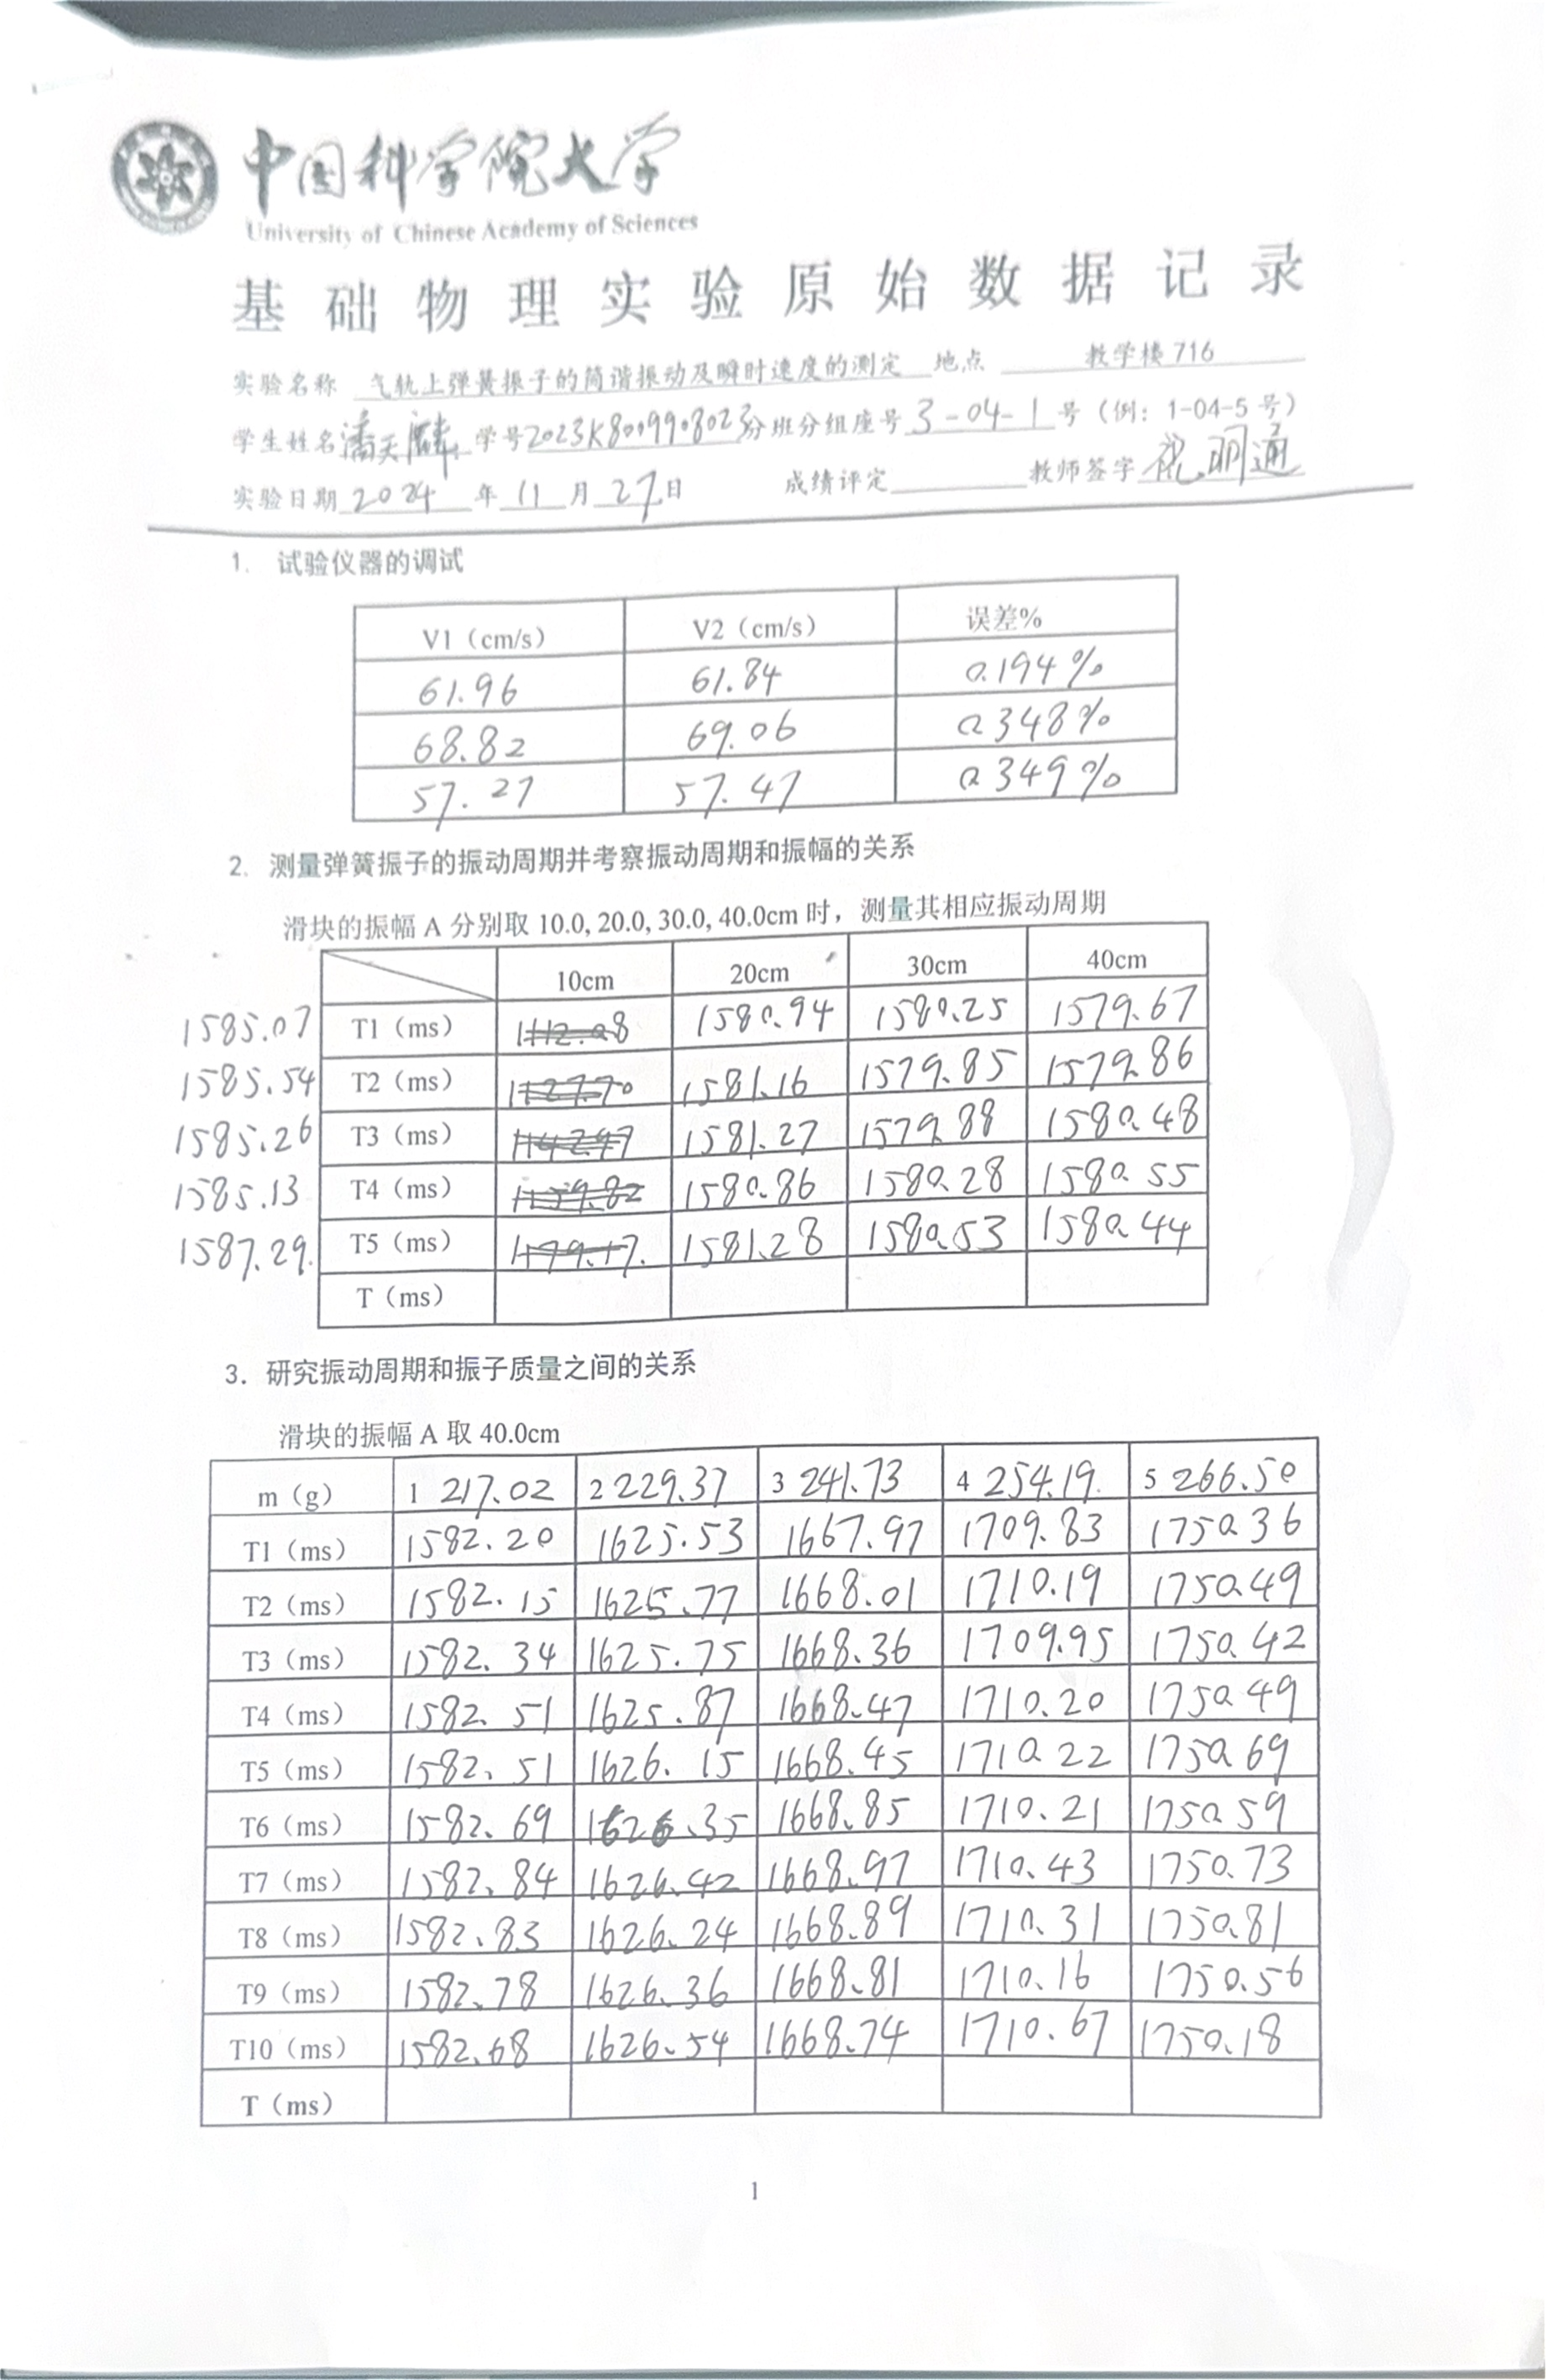
\includepdf[pages=-]{潘天麟-气轨试验-数据.pdf}
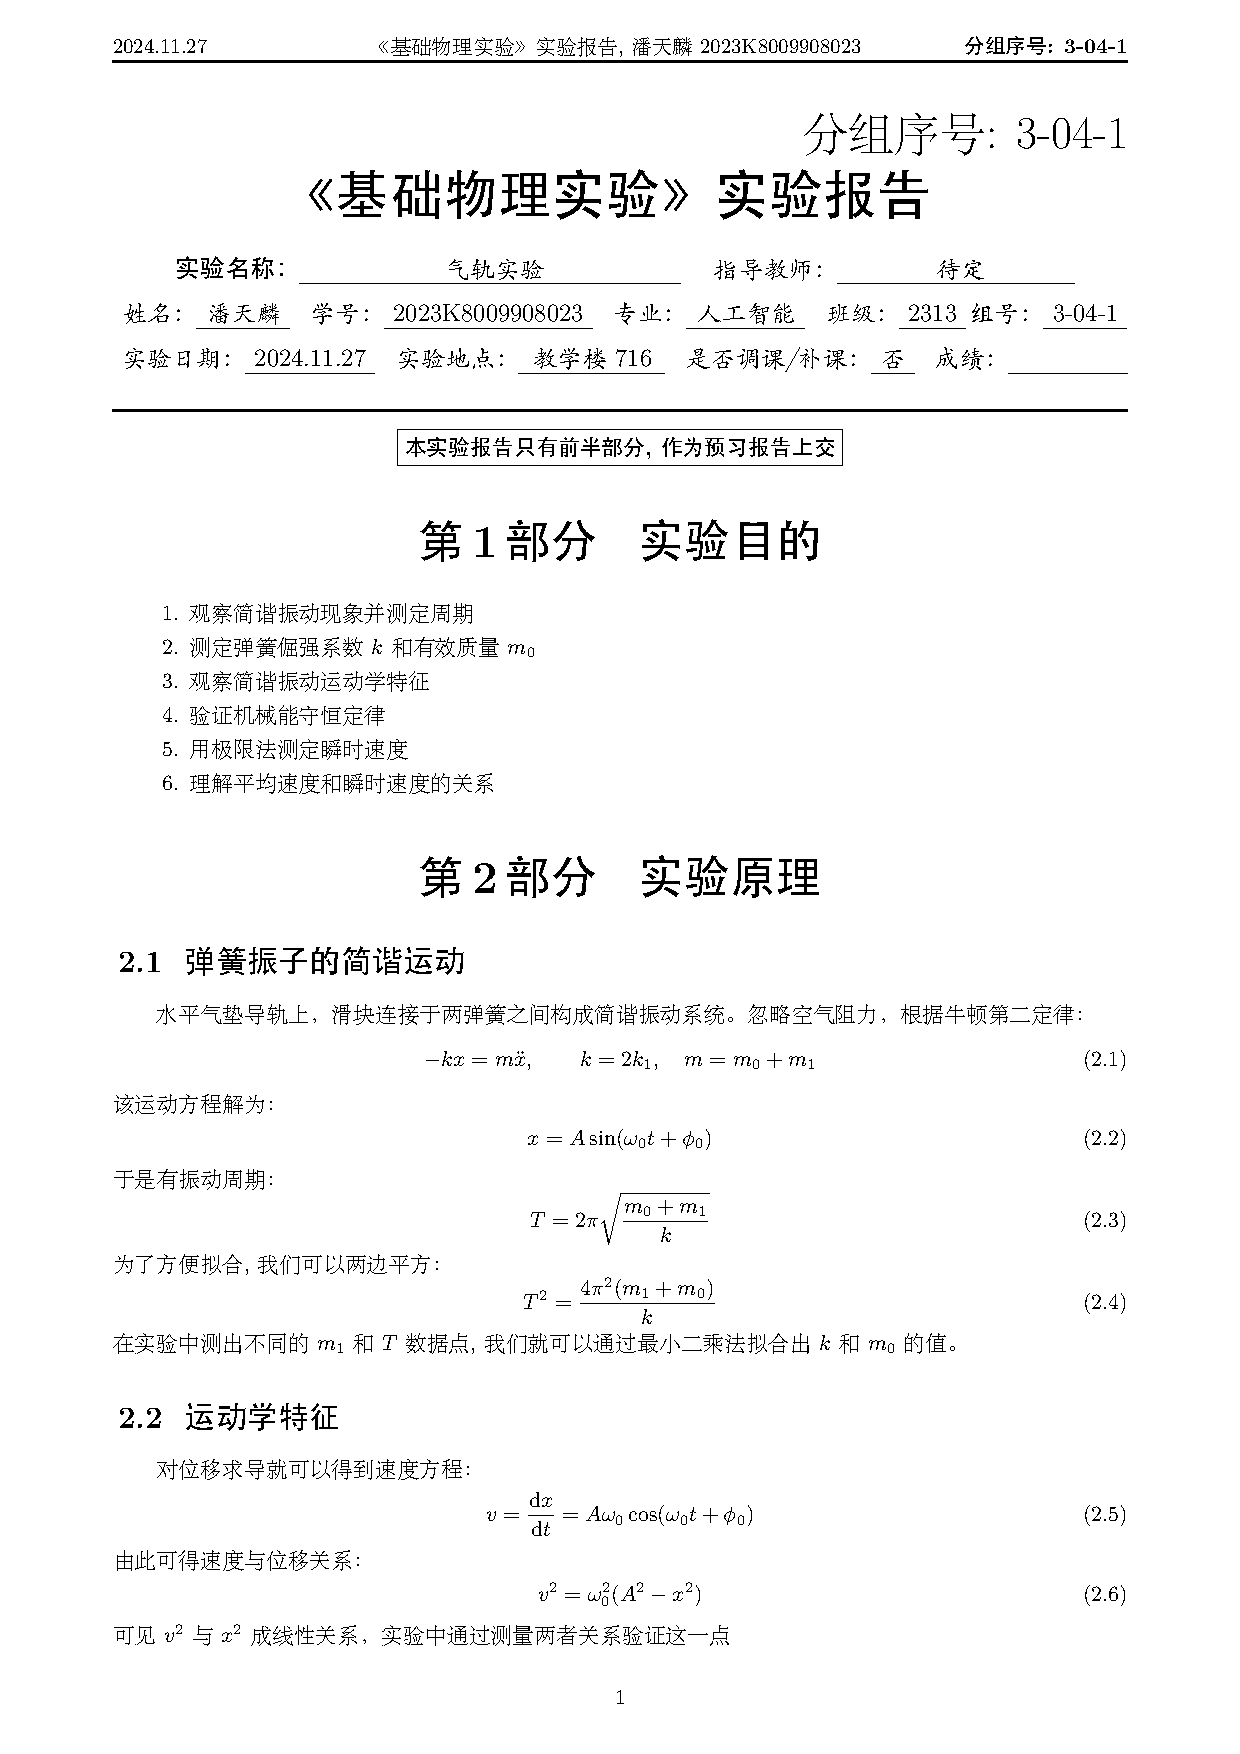
\includepdf[pages=-]{潘天麟-2024-11-27-气轨实验-预习报告.pdf}


\end{document}

